\documentclass[lualatex,handout]{beamer}
\setbeamertemplate{footline}[frame number]
%\useoutertheme{infolines}
\usepackage{luatexja}
\usepackage{amsmath,amssymb}
\usepackage{mathtools}

\usepackage{tikz}
\usepackage{pgfplots}

%\usepackage[haranoaji]{luatexja-preset}
\usepackage[deluxe,ipaex]{luatexja-preset}
\renewcommand{\kanjifamilydefault}{\gtdefault}
%\setmainjfont{HaranoAjiGothic-Regular}

\usepackage{unicode-math}
%\setmathfont{Fira Math}
\setmathfont{STIX Two Math}
\setmathrm{STIX Two Math}[StylisticSet=8]
%\setmathfont{STIX Two Math}[range={up,it,bb,bbit,scr,bfscr},StylisticSet=8]
%\setmathfont{XITS Math}
%\setmathrm{XITS Math}[StylisticSet=8]
%\setmathfont{XITS Math}[StylisticSet=8]

%\usefonttheme{professionalfonts}

\usepackage{luacolor}

\newcommand{\emm}[1]{\textcolor{red}{#1}}
\newcommand{\expt}[1]{\mathbb{E}\left[#1\right]}
\newcommand{\var}[1]{\mathbb{V}\left[#1\right]}
\newcommand{\cov}[1]{\mathrm{Cov}\left[#1\right]}


\usepackage{xspace}
\newcommand\bm[1]{{\mathbf{#1}}}

\theoremstyle{definition}

\title{確率・統計基礎: 確率論の初歩のおさらい}
\author{森 立平}
\date{}



\begin{document}
\begin{frame}[plain]
\maketitle
\end{frame}


\begin{frame}{確率とは}
\begin{itemize}
\setlength{\itemsep}{2em}
\item 世の中のランダムな事象を数学的に記述したもの
\item 統計・機械学習の基礎となっている
\item 極限定理: 確率$p$で表が出るコインを$N$回投げた時に、表が出る回数$F$は
\vspace{1em}
\begin{itemize}
\setlength{\itemsep}{1em}
\item 大数の法則: $\frac{F}{N} \to p$
\item 大偏差原理: $\Pr\left(\left|\frac{F}{N} - p\right| > \epsilon\right) = \mathrm{e}^{-\beta N}$
\item 中心極限定理: $\frac{F-pN}{\sqrt{N}}\to$正規分布
\end{itemize}
\end{itemize}
\end{frame}

\begin{frame}{統計とは}
確率論は統計の基礎となる
\vspace{1em}
\begin{itemize}
\item クラスタリング: この患者は病気ですか?
\item a
\end{itemize}
\end{frame}

\begin{frame}{確率論の数学モデルとは?}
\begin{center}
\large 測度論!
\end{center}

\vspace{1em}
\begin{itemize}
\setlength{\itemsep}{2em}
\item 確率は面積($=$測度)のようなもの。
\item 数学的に\textbf{厳密}に様々な結果(大数の法則、大偏差原理、中心極限定理)が証明できる。
\item とても重要だが勉強するのは3年生以降(解析学要論Ⅱ、確率論)。
\item この授業では測度論を使わない代わりに\emm{制限された確率論}をやる。
\end{itemize}
\end{frame}

\begin{frame}{確率論の公理}
\emm{確率空間} $(\Omega, \mathcal{F}, P)$

\vspace{.5em}
\begin{itemize}
\item $\Omega\colon$ 集合(\emm{標本空間})
\item $\mathcal{F}\subseteq 2^\Omega$ (\emm{事象の集合}、可測集合)
\item $P\colon\mathcal{F}\to[0,1]$ (\emm{確率測度})
\end{itemize}

\vspace{.5em}
可測集合の公理($\sigma$-加法族、完全加法族)
\begin{enumerate}
\item $\emptyset\in\mathcal{F}$.
\item $A\in\mathcal{F}\Longrightarrow A^c\in\mathcal{F}$.
\item $A,\,B\in\mathcal{F}\Longrightarrow A\cup B\in\mathcal{F}$ (有限加法性).
\item[3'.] $(A_n\in\mathcal{F})_{n=1,\dotsc}\Longrightarrow \bigcup_{n=1}^\infty A_n\in\mathcal{F}$ (完全加法性).
\end{enumerate}

\vspace{.5em}
確率の公理
\begin{enumerate}
\item $P(\Omega)=1$.
\item $\forall A, B\in\mathcal{F}$, $A\cup B=\emptyset\Longrightarrow P(A\cup B)=P(A)+P(B)$\\ (有限加法性).
\item[2'.] $\forall (A_n\in\mathcal{F})_{n=1,\dotsc}$, $\forall i\ne j,\, A_i\cup A_j=\emptyset\Longrightarrow P\left(\bigcup_{n=1}^\infty A_n\right)=\sum_{n=1}^\infty P(A_n)$\\ (完全加法性).
\end{enumerate}
\end{frame}

\begin{frame}{無限個の集合の操作}
\end{frame}

\begin{frame}{なぜ有限加法性じゃ駄目なの?$\leftarrow$駄目じゃないけど$\dotsc$}
\begin{theorem}[確率測度の連続性]
$P$を\emm{完全加法}確率測度とする。
事象$A_1\subseteq A_2\subseteq \dotsb$について
\begin{align*}
P\left(\bigcup_{i=1}^\infty A_i\right) = \lim_{n\to\infty} P(A_n).
\end{align*}
\end{theorem}
\begin{proof}
$B_1\coloneq A_1$, $i\ge 2$について$B_i\coloneq A_i\setminus A_{i-1}$とおく。
このとき、$i\ne j$について $B_i\cap B_j=\emptyset$。また、$\bigcup_{i=1}^n B_i = \bigcup_{i=1}^nA_i$.
\begin{align*}
P\left(\bigcup_{i=1}^\infty A_i\right)&= P\left(\bigcup_{i=1}^\infty B_i\right) =\sum_{i=1}^\infty P(B_i)\\
&=\lim_{n\to\infty} \sum_{i=1}^n P(B_i)
=\lim_{n\to\infty} P\left(\bigcup_{i=1}^n B_i\right)
=\lim_{n\to\infty} P(A_n).\qedhere
\end{align*}
\end{proof}
\end{frame}

\begin{frame}{確率空間の例}
離散的な分布
\begin{itemize}
\item $\Omega\colon$ 有限集合 or 可算無限集合.
\item $\mathcal{F} = 2^\Omega$.
\item $P(A) = \sum_{k\in A} P(\{k\})$ ここで $\sum_{k\in\Omega} P(\{k\})=1$.
\end{itemize}

\vspace{1em}
\begin{itemize}
\item $\Omega=[0,1)\subseteq\mathbb{R}$
\item $\mathcal{F} = $すべての閉区間を含む
\item $P([a,b]) = b-a$.
\end{itemize}

\end{frame}

\begin{frame}{$\mathcal{F} = 2^\Omega$にしたいです$\leftarrow$無理です(完全加法性+選択公理)}
\small
確率空間$(\Omega,\mathcal{F},P)$が以下を満たすとする
\begin{itemize}
\item $\Omega=[0,1)$, $\mathcal{F} = 2^\Omega$.
%\item $P([a,b]) = b-a$.
\item $\forall c\in\Omega,\, A\in\mathcal{F},\, P(A+c) = P(A)$ where $A+c\coloneq\{a+c-\lfloor a+c\rfloor\mid a\in A\}$.
\end{itemize}
\emm{選択公理を仮定するとそのような確率空間は存在しない}。

\vspace{1em}
$\Omega$の上の同値関係を
$x\sim y\stackrel{\mathrm{def}}{\iff} x-y \in\mathbb{Q}$と定義する。

\vspace{1em}
$\Omega$の上の同値類から一つずつ要素を選んで集合$V$を作る(選択公理)。
%
\begin{align*}
1 = P([0,1)) &= P\left(\bigcup_{x\in\mathbb{Q}} (V + x)\right)\\
&= \sum_{x\in\mathbb{Q}} P\left(V + x\right)\qquad\text{(完全加法性)}\\
&= \sum_{x\in\mathbb{Q}} P\left(V\right)
\end{align*}
同じ値を無限回足して1にはできない。
\end{frame}

\if0
\begin{frame}{離散的な確率分布}
有限集合$\{1,2,\dotsc,n\}$上の確率分布
\begin{itemize}
\item $p_1, p_2, \dotsc, p_n\ge 0$, $p_1+p_2+\dotsb+p_n=0$.
\item $\mathrm{abc}$
\end{itemize}
\end{frame}
\fi

\begin{frame}{確率変数}
$X\colon $
\begin{align*}
\Pr(X\ge a)
\end{align*}
\end{frame}

\begin{frame}{離散確率分布の例}
\begin{itemize}
\setlength{\itemsep}{1em}
\item 二項分布: {\small $n$回独立にコインを投げて$k$回表が出る確率}\\
$\Pr(X = k) = \binom{n}{k} p^k(1-p)^{n-k}$.
\item 幾何分布: {\small 独立にコインを投げて$k$回目に初めて表が出る確率}\\
$\Pr(X = k) = (1-p)^{k-1}p$.
\item {\small 負の二項分布: 独立にコインを投げて$r$回表が出る前にちょうど$k$回裏が出る確率}\\
$\Pr(X = k) = \binom{r+k-1}{r-1}p^r(1-p)^k$.
\item 超幾何分布: {\small 袋の中に$N$個のボールがあって、そのうち$K$個が当たりのとき、$n$個引いて$k$個当たりを引く確率}\\
$\Pr(X = k) = \frac{\binom{K}{k}\binom{N-K}{n-k}}{\binom{N}{n}}$. 
\item ポアソン分布:
$\Pr(X = k) = \frac{\lambda^k}{k!} \mathrm{e}^{-\lambda}$
\end{itemize}
\end{frame}

\begin{frame}{二項分布}
\begin{align*}
\Pr(X = k) &= \binom{n}{k} p^k(1-p)^{n-k},\quad n=30,\, p=0.3.
\end{align*}
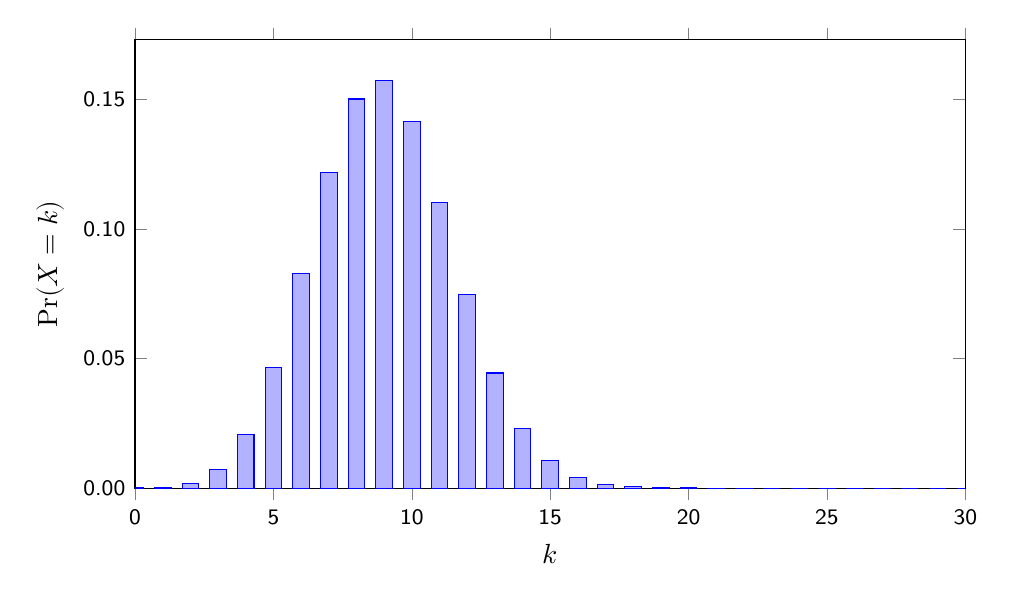
\begin{tikzpicture}[%
declare function={binom(\k,\n,\p)=\n!/(\k!*(\n-\k)!)*\p^\k*(1-\p)^(\n-\k);}]
\pgfmathsetmacro{\binomN}{30}
\begin{axis}[
    width=\textwidth, height=\axisdefaultheight,
    ylabel={$\Pr(X=k)$},
    xlabel={$k$},
    xmin=0, xmax=\binomN,
    ymin=0,
    scaled ticks = false,
    tick label style={/pgf/number format/assume math mode=true, font=\footnotesize\sffamily},
    yticklabel style={/pgf/number format/.cd, fixed, fixed zerofill, precision=2},
        domain=0:\binomN,samples at={0,1,...,\binomN},
    mark options={scale=0.75, blue},
    ybar, bar width = 6pt
        ]
%\addplot[ycomb] {binom(x,\binomN,0.3)};
\addplot {binom(x,\binomN,0.3)};
\end{axis}
\end{tikzpicture}
\end{frame}

\begin{frame}{幾何分布}
\begin{align*}
\Pr(X = k) &= (1-p)^{k-1}p,\quad p=0.3.
\end{align*}
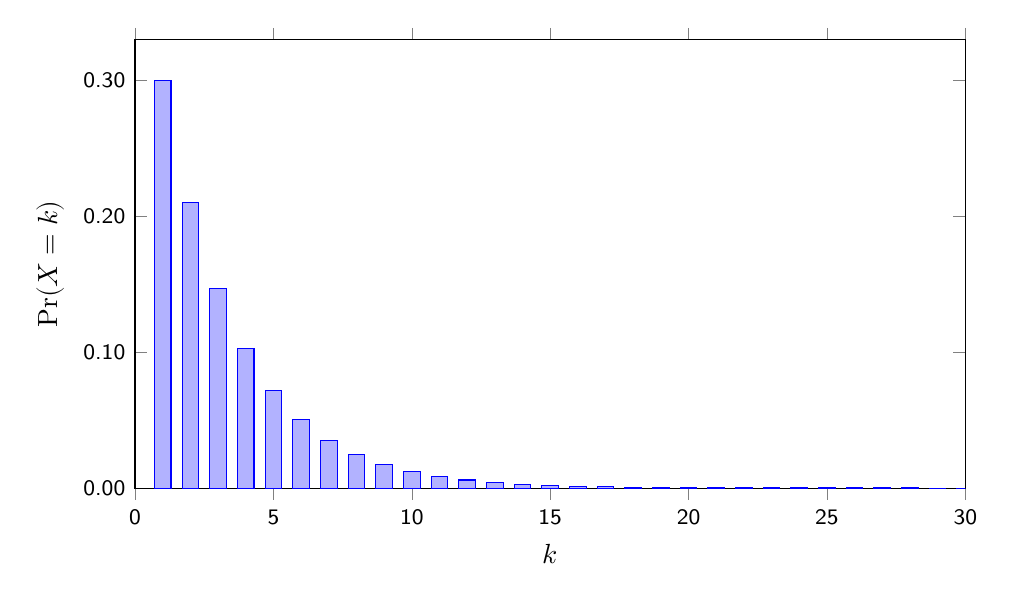
\begin{tikzpicture}[%
declare function={geom(\k,\p)=(1-\p)^(\k-1)*\p;}]
\pgfmathsetmacro{\XMAX}{30}
\begin{axis}[
    width=\textwidth, height=\axisdefaultheight,
    ylabel={$\Pr(X=k)$},
    xlabel={$k$},
    xmin=0, xmax=\XMAX,
    ymin=0,
    scaled ticks = false,
    tick label style={/pgf/number format/assume math mode=true, font=\footnotesize\sffamily},
    yticklabel style={/pgf/number format/.cd, fixed, fixed zerofill, precision=2},
        domain=1:\XMAX,samples at={1,2,...,\XMAX},
    mark options={scale=0.75, blue},
    ybar, bar width = 6pt
        ]
%\addplot[ycomb] {binom(x,\binomN,0.3)};
\addplot {geom(x,0.3)};
\end{axis}
\end{tikzpicture}
\end{frame}

\begin{frame}{負の二項分布}
\begin{align*}
\Pr(X = k) = \binom{r+k-1}{r-1}p^r(1-p)^k,\quad r=5,\, p=0.3.
\end{align*}
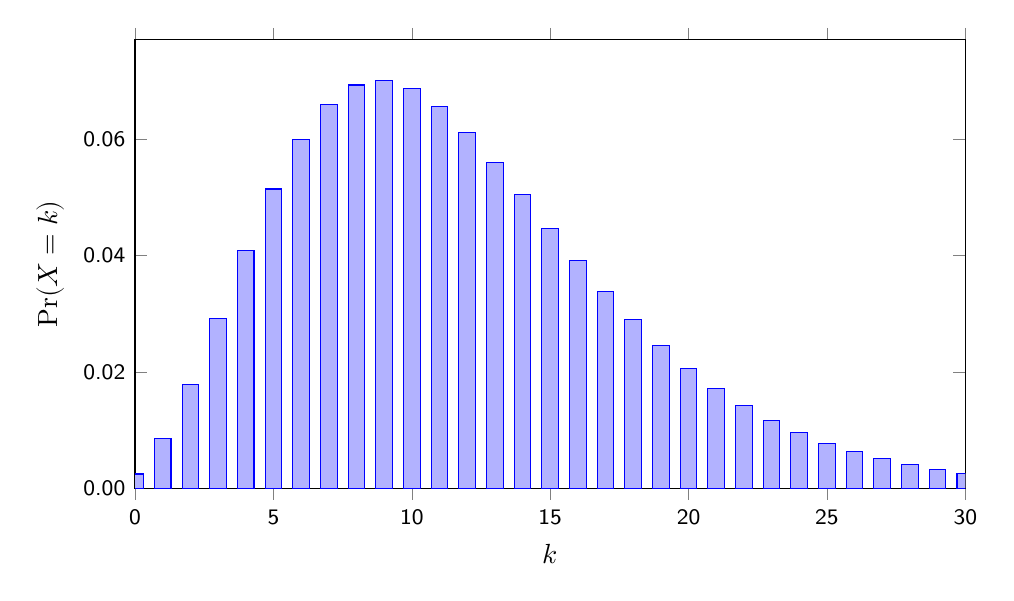
\begin{tikzpicture}[%
declare function={nbinom(\k,\r,\p)=(\r+\k-1)!/(\k!*(\r-1)!)*\p^\r*(1-\p)^\k;}]
\pgfmathsetmacro{\XMAX}{30}
\begin{axis}[
    width=\textwidth, height=\axisdefaultheight,
    ylabel={$\Pr(X=k)$},
    xlabel={$k$},
    xmin=0, xmax=\XMAX,
    ymin=0,
    scaled ticks = false,
    tick label style={/pgf/number format/assume math mode=true, font=\footnotesize\sffamily},
    yticklabel style={/pgf/number format/.cd, fixed, fixed zerofill, precision=2},
        domain=0:\XMAX,samples at={0,1,...,\XMAX},
    mark options={scale=0.75, blue},
    ybar, bar width = 6pt
        ]
%\addplot[ycomb] {binom(x,\binomN,0.3)};
\addplot {nbinom(x,5,0.3)};
\end{axis}
\end{tikzpicture}
\end{frame}

\begin{frame}{超幾何分布}

\vspace{-1em}
\begin{align*}
\Pr(X = k) = \frac{\binom{K}{k}\binom{N-K}{n-k}}{\binom{N}{n}},\quad N=100,\, K=30,\, n=40. 
\end{align*}
%\vfill
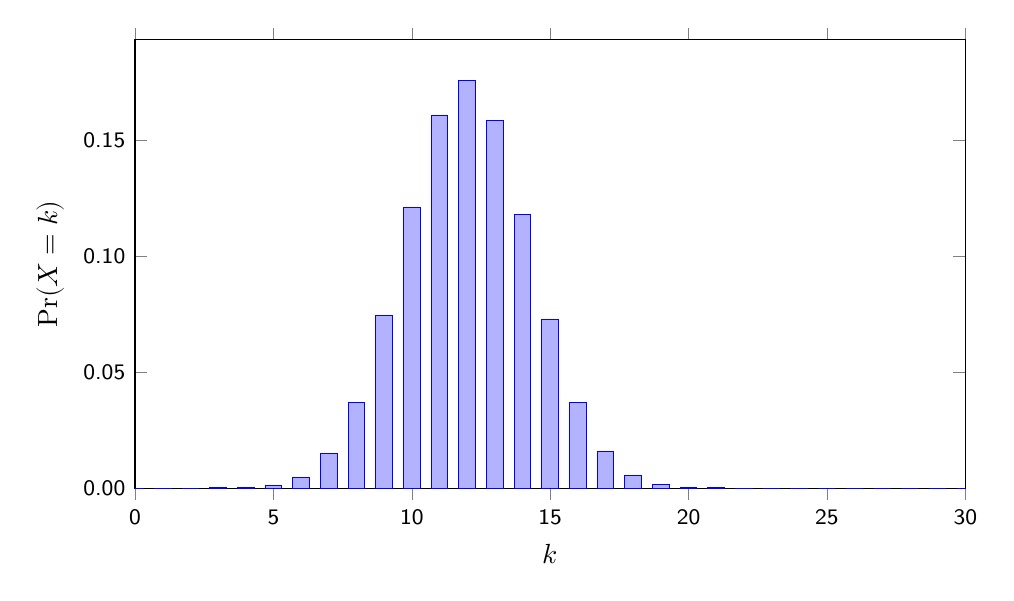
\begin{tikzpicture}[%
declare function={binom(\N,\K)=\N!/(\K!*(\N-\K)!);},
declare function={hypgeom(\k,\N,\K,\n)=binom(\K,\k)*binom(\N-\K,\n-\k)/binom(\N,\n);}]
\pgfmathsetmacro{\XMAX}{30}
\begin{axis}[
    width=\textwidth, height=\axisdefaultheight,
    ylabel={$\Pr(X=k)$},
    xlabel={$k$},
    xmin=0, xmax=\XMAX,
    ymin=0,
    scaled ticks = false,
    tick label style={/pgf/number format/assume math mode=true, font=\footnotesize\sffamily},
    yticklabel style={/pgf/number format/.cd, fixed, fixed zerofill, precision=2},
        domain=0:\XMAX,samples at={0,1,...,\XMAX},
    mark options={scale=0.75, blue},
    ybar, bar width = 6pt
        ]
%\addplot[ycomb] {binom(x,\binomN,0.3)};
\addplot {hypgeom(x,100,\XMAX,40)};
\end{axis}
\end{tikzpicture}
\end{frame}

\begin{frame}{ポアソン分布}
\begin{align*}
\Pr(X = k) &= \frac{\lambda^k}{k!} \mathrm{e}^{-\lambda},\quad\lambda=10
\end{align*}
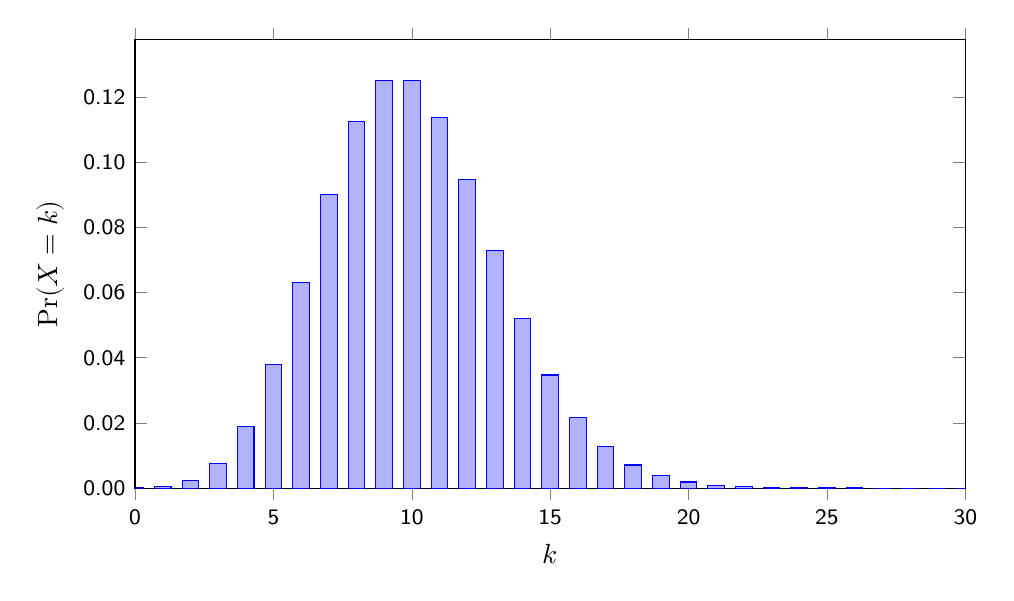
\begin{tikzpicture}[%
declare function={poisson(\k,\l)=\l^\k/\k!*exp(-\l);}]
\pgfmathsetmacro{\XMAX}{30}
\begin{axis}[
    width=\textwidth, height=\axisdefaultheight,
    ylabel={$\Pr(X=k)$},
    xlabel={$k$},
    xmin=0, xmax=\XMAX,
    ymin=0,
    scaled ticks = false,
    tick label style={/pgf/number format/assume math mode=true, font=\footnotesize\sffamily},
    yticklabel style={/pgf/number format/.cd, fixed, fixed zerofill, precision=2},
        domain=0:\XMAX,samples at={0,1,...,\XMAX},
    mark options={scale=0.75, blue},
    ybar, bar width = 6pt
        ]
%\addplot[ycomb] {binom(x,\binomN,0.3)};
\addplot {poisson(x,10)};
\end{axis}
\end{tikzpicture}
\end{frame}


\begin{frame}{同時確率と条件付き確率}
確率変数$X$と$Y$の同時確率
\begin{align*}
\Pr(X=x, Y=y)
\end{align*}
周辺化
\begin{align*}
\Pr(X=x) &= \sum_y \Pr(X=x, Y=y)\\
\Pr(Y=y) &= \sum_x \Pr(X=x, Y=y)
\end{align*}

条件付確率
\begin{align*}
\Pr(X=x\mid Y=y) &= \frac{\Pr(X=x,Y=y)}{\Pr(Y=y)}
\end{align*}
\small $Y=y$のときの$X=x$の確率($\Pr(Y=y)=0$のときは定義されない)
\end{frame}

\begin{frame}{独立確率変数}
確率変数$X$と$Y$が独立$\stackrel{\mathrm{def}}{\iff}\Pr(X=x,Y=y)=\Pr(X=x)\Pr(Y=y)$.

\vspace{2em}
任意の写像$f$と$g$について、

確率変数$X$と$Y$が独立$\Longrightarrow$ $f(X)$と$g(Y)$は独立。
\end{frame}

\begin{frame}{期待値}
\begin{align*}
\expt{X} &= \sum_k \Pr(X=k) k
\end{align*}
線形
\begin{align*}
\expt{aX + bY} &= \sum_k \Pr(aX+bY=k) k\\
&= \sum_{x, y} \Pr(X=x, Y=y) (ax+by)\\
&= \sum_{x, y} \Pr(X=x, Y=y) ax + \sum_{x, y} \Pr(X=x, Y=y) by\\
&= \sum_{x} \Pr(X=x) ax + \sum_{y} \Pr(Y=y) by\\
&= a\sum_{x} \Pr(X=x) x + b\sum_{y} \Pr(Y=y) y\\
&=a\expt{X} + b\expt{Y} 
\end{align*}
\end{frame}

\begin{frame}{期待値の例}

\end{frame}


\begin{frame}{マルコフの不等式}
\begin{theorem}[マルコフの不等式]
任意の\emm{非負}の確率変数$X$と$a>0$について
\begin{align*}
\Pr(X\ge a) &\le \frac{\expt{X}}{a}
\end{align*}
\end{theorem}
\begin{proof}
\vspace{-2em}
\begin{align*}
\expt{X} &= \sum_i p_i x_i\\
&= \sum_{i\colon x_i \ge a} p_i x_i
+ \sum_{i\colon x_i < a} p_i x_i\\
&\ge \sum_{i\colon x_i \ge a} p_i x_i\hspace{8em}(x_i\ge 0)\\
&\ge \sum_{i\colon x_i \ge a} p_i a\\
&= a\Pr(X\ge a) \qedhere
\end{align*}
\end{proof}
\end{frame}

\begin{frame}{例題}
\end{frame}

\begin{frame}{分散}
\begin{align*}
\var{X} &= \expt{(X-\expt{X})^2}\\
&=\expt{X^2-2X\expt{X}+\expt{X}^2}\\
&=\expt{X^2}-2\expt{X}\expt{X}+\expt{X}^2\\
&=\emm{\expt{X^2}-\expt{X}^2}\\
\end{align*}
\begin{center}
分散は\emm{非負}で\emm{期待値からの広がり}を表す量。
\end{center}
\end{frame}

\begin{frame}{分散の意味}
\begin{align*}
\var{X} &= \expt{(X-\expt{X})^2}
\end{align*}

$\var{X} = 0 \iff \Pr(X = \expt{X})=1$.
\end{frame}

\begin{frame}{分散の性質}
\small
\begin{align*}
\var{X} &= \expt{(X-\expt{X})^2}
\end{align*}
%\vspace{1em}
\begin{align*}
\var{aX} &= \expt{(aX-\expt{aX})^2}\\
&= \expt{(aX-a\expt{X})^2}\\
&= \expt{a^2(X-\expt{X})^2}\\
&= a^2\expt{(X-\expt{X})^2}\\
&= a^2\var{X}
\end{align*}
%
\begin{align*}
\var{X+Y} &= \expt{(X+Y-\expt{X+Y})^2}\\
 &= \expt{(X-\expt{X}+Y-\expt{Y})^2}\\
 &= \expt{(X-\expt{X})^2+(Y-\expt{Y})^2 + 2(X-\expt{X})(Y-\expt{Y})}\\
 &= \expt{(X-\expt{X})^2}+\expt{(Y-\expt{Y})^2} + 2\expt{(X-\expt{X})(Y-\expt{Y})}\\
 &= \var{X}+\var{Y}+ 2\emm{\expt{(X-\expt{X})(Y-\expt{Y})}}\\
\end{align*}
\end{frame}

\begin{frame}{共分散}
\begin{align*}
\cov{X,Y} &= \expt{(X-\expt{X})(Y-\expt{Y})}
\end{align*}

\vspace{1em}

\begin{itemize}
\setlength{\itemsep}{2em}
\item $X-\expt{X}$と$Y-\expt{Y}$の符号が一緒 $\Rightarrow$ $\cov{X,Y}\ge 0$。
\item $X-\expt{X}$と$Y-\expt{Y}$の符号が逆 $\Rightarrow$ $\cov{X,Y}\le 0$。
\end{itemize}

\vspace{1em}
直感的な意味

\vspace{1em}
\begin{itemize}
\setlength{\itemsep}{2em}
\item $X$が大きいとき$Y$が大きい $\Rightarrow$ $\cov{X,Y}\ge 0$。
\item $X$が大きいとき$Y$が小さい $\Rightarrow$ $\cov{X,Y}\ge 0$。
\end{itemize}
\end{frame}

\begin{frame}{無相関と独立}
\begin{align*}
\cov{X,Y} &= \expt{(X-\expt{X})(Y-\expt{Y})} = 0
\end{align*}
\end{frame}

\begin{frame}{チェビシェフの不等式}
\begin{lemma}[チェビシェフの不等式]
確率変数$X$が分散を持つと仮定する。任意の $a>0$について
\begin{align*}
\Pr(|X-\expt{X}|\ge a) &\le \frac{\var{X}}{a^2}
\end{align*}
\end{lemma}
\begin{proof}
\begin{align*}
\Pr(|X-\expt{X}|\ge a) &=\Pr((X-\expt{X})^2\ge a^2)\\
&\le\frac{\expt{(X-\expt{X})^2}}{a^2}\hspace{3em}\text{(マルコフの不等式)}
\end{align*}
\end{proof}
\end{frame}

\begin{frame}{コーシー・シュワルツの不等式}
\begin{theorem}
\begin{align*}
\expt{XY}^2 \le \expt{X^2}\expt{Y^2}
\end{align*}
\end{theorem}
\end{frame}

\begin{frame}{イェンセンの不等式}
\begin{theorem}
凸関数$f\colon\mathbb{R}\to\mathbb{R}$について
\begin{align*}
\expt{f(X)} \ge f(\expt{X})
\end{align*}
\end{theorem}

\end{frame}

\end{document}
